% Created by tikzDevice version 0.12 on 2019-06-13 16:13:38
% !TEX encoding = UTF-8 Unicode
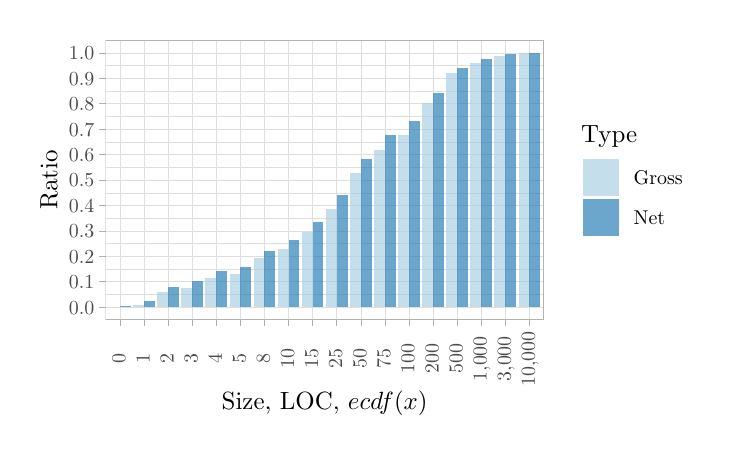
\begin{tikzpicture}[x=1pt,y=1pt]
\definecolor{fillColor}{RGB}{255,255,255}
\path[use as bounding box,fill=fillColor,fill opacity=0.00] (0,0) rectangle (245.72,144.54);
\begin{scope}
\path[clip] (  0.00,  0.00) rectangle (245.72,144.54);
\definecolor{drawColor}{RGB}{255,255,255}
\definecolor{fillColor}{RGB}{255,255,255}

\path[draw=drawColor,line width= 0.5pt,line join=round,line cap=round,fill=fillColor] (  0.00,  0.00) rectangle (245.72,144.54);
\end{scope}
\begin{scope}
\path[clip] ( 28.14, 38.94) rectangle (186.52,140.04);
\definecolor{fillColor}{RGB}{255,255,255}

\path[fill=fillColor] ( 28.14, 38.94) rectangle (186.52,140.04);
\definecolor{drawColor}{gray}{0.87}

\path[draw=drawColor,line width= 0.1pt,line join=round] ( 28.14, 38.94) --
	(186.52, 38.94);

\path[draw=drawColor,line width= 0.1pt,line join=round] ( 28.14, 48.13) --
	(186.52, 48.13);

\path[draw=drawColor,line width= 0.1pt,line join=round] ( 28.14, 57.32) --
	(186.52, 57.32);

\path[draw=drawColor,line width= 0.1pt,line join=round] ( 28.14, 66.51) --
	(186.52, 66.51);

\path[draw=drawColor,line width= 0.1pt,line join=round] ( 28.14, 75.70) --
	(186.52, 75.70);

\path[draw=drawColor,line width= 0.1pt,line join=round] ( 28.14, 84.89) --
	(186.52, 84.89);

\path[draw=drawColor,line width= 0.1pt,line join=round] ( 28.14, 94.08) --
	(186.52, 94.08);

\path[draw=drawColor,line width= 0.1pt,line join=round] ( 28.14,103.28) --
	(186.52,103.28);

\path[draw=drawColor,line width= 0.1pt,line join=round] ( 28.14,112.47) --
	(186.52,112.47);

\path[draw=drawColor,line width= 0.1pt,line join=round] ( 28.14,121.66) --
	(186.52,121.66);

\path[draw=drawColor,line width= 0.1pt,line join=round] ( 28.14,130.85) --
	(186.52,130.85);

\path[draw=drawColor,line width= 0.1pt,line join=round] ( 28.14,140.04) --
	(186.52,140.04);

\path[draw=drawColor,line width= 0.2pt,line join=round] ( 28.14, 43.53) --
	(186.52, 43.53);

\path[draw=drawColor,line width= 0.2pt,line join=round] ( 28.14, 52.72) --
	(186.52, 52.72);

\path[draw=drawColor,line width= 0.2pt,line join=round] ( 28.14, 61.92) --
	(186.52, 61.92);

\path[draw=drawColor,line width= 0.2pt,line join=round] ( 28.14, 71.11) --
	(186.52, 71.11);

\path[draw=drawColor,line width= 0.2pt,line join=round] ( 28.14, 80.30) --
	(186.52, 80.30);

\path[draw=drawColor,line width= 0.2pt,line join=round] ( 28.14, 89.49) --
	(186.52, 89.49);

\path[draw=drawColor,line width= 0.2pt,line join=round] ( 28.14, 98.68) --
	(186.52, 98.68);

\path[draw=drawColor,line width= 0.2pt,line join=round] ( 28.14,107.87) --
	(186.52,107.87);

\path[draw=drawColor,line width= 0.2pt,line join=round] ( 28.14,117.06) --
	(186.52,117.06);

\path[draw=drawColor,line width= 0.2pt,line join=round] ( 28.14,126.25) --
	(186.52,126.25);

\path[draw=drawColor,line width= 0.2pt,line join=round] ( 28.14,135.44) --
	(186.52,135.44);

\path[draw=drawColor,line width= 0.2pt,line join=round] ( 33.36, 38.94) --
	( 33.36,140.04);

\path[draw=drawColor,line width= 0.2pt,line join=round] ( 42.06, 38.94) --
	( 42.06,140.04);

\path[draw=drawColor,line width= 0.2pt,line join=round] ( 50.77, 38.94) --
	( 50.77,140.04);

\path[draw=drawColor,line width= 0.2pt,line join=round] ( 59.47, 38.94) --
	( 59.47,140.04);

\path[draw=drawColor,line width= 0.2pt,line join=round] ( 68.17, 38.94) --
	( 68.17,140.04);

\path[draw=drawColor,line width= 0.2pt,line join=round] ( 76.87, 38.94) --
	( 76.87,140.04);

\path[draw=drawColor,line width= 0.2pt,line join=round] ( 85.57, 38.94) --
	( 85.57,140.04);

\path[draw=drawColor,line width= 0.2pt,line join=round] ( 94.28, 38.94) --
	( 94.28,140.04);

\path[draw=drawColor,line width= 0.2pt,line join=round] (102.98, 38.94) --
	(102.98,140.04);

\path[draw=drawColor,line width= 0.2pt,line join=round] (111.68, 38.94) --
	(111.68,140.04);

\path[draw=drawColor,line width= 0.2pt,line join=round] (120.38, 38.94) --
	(120.38,140.04);

\path[draw=drawColor,line width= 0.2pt,line join=round] (129.08, 38.94) --
	(129.08,140.04);

\path[draw=drawColor,line width= 0.2pt,line join=round] (137.79, 38.94) --
	(137.79,140.04);

\path[draw=drawColor,line width= 0.2pt,line join=round] (146.49, 38.94) --
	(146.49,140.04);

\path[draw=drawColor,line width= 0.2pt,line join=round] (155.19, 38.94) --
	(155.19,140.04);

\path[draw=drawColor,line width= 0.2pt,line join=round] (163.89, 38.94) --
	(163.89,140.04);

\path[draw=drawColor,line width= 0.2pt,line join=round] (172.59, 38.94) --
	(172.59,140.04);

\path[draw=drawColor,line width= 0.2pt,line join=round] (181.30, 38.94) --
	(181.30,140.04);
\definecolor{fillColor}{RGB}{31,120,180}

\path[fill=fillColor,fill opacity=0.66] ( 33.36, 43.53) rectangle ( 37.28, 43.85);
\definecolor{fillColor}{RGB}{166,206,227}

\path[fill=fillColor,fill opacity=0.66] ( 29.45, 43.53) rectangle ( 33.36, 43.53);
\definecolor{fillColor}{RGB}{31,120,180}

\path[fill=fillColor,fill opacity=0.66] ( 42.06, 43.53) rectangle ( 45.98, 45.69);
\definecolor{fillColor}{RGB}{166,206,227}

\path[fill=fillColor,fill opacity=0.66] ( 38.15, 43.53) rectangle ( 42.06, 44.41);
\definecolor{fillColor}{RGB}{31,120,180}

\path[fill=fillColor,fill opacity=0.66] ( 50.77, 43.53) rectangle ( 54.68, 50.73);
\definecolor{fillColor}{RGB}{166,206,227}

\path[fill=fillColor,fill opacity=0.66] ( 46.85, 43.53) rectangle ( 50.77, 49.05);
\definecolor{fillColor}{RGB}{31,120,180}

\path[fill=fillColor,fill opacity=0.66] ( 59.47, 43.53) rectangle ( 63.38, 52.97);
\definecolor{fillColor}{RGB}{166,206,227}

\path[fill=fillColor,fill opacity=0.66] ( 55.55, 43.53) rectangle ( 59.47, 50.57);
\definecolor{fillColor}{RGB}{31,120,180}

\path[fill=fillColor,fill opacity=0.66] ( 68.17, 43.53) rectangle ( 72.09, 56.49);
\definecolor{fillColor}{RGB}{166,206,227}

\path[fill=fillColor,fill opacity=0.66] ( 64.25, 43.53) rectangle ( 68.17, 53.93);
\definecolor{fillColor}{RGB}{31,120,180}

\path[fill=fillColor,fill opacity=0.66] ( 76.87, 43.53) rectangle ( 80.79, 57.93);
\definecolor{fillColor}{RGB}{166,206,227}

\path[fill=fillColor,fill opacity=0.66] ( 72.96, 43.53) rectangle ( 76.87, 55.69);
\definecolor{fillColor}{RGB}{31,120,180}

\path[fill=fillColor,fill opacity=0.66] ( 85.57, 43.53) rectangle ( 89.49, 63.93);
\definecolor{fillColor}{RGB}{166,206,227}

\path[fill=fillColor,fill opacity=0.66] ( 81.66, 43.53) rectangle ( 85.57, 61.13);
\definecolor{fillColor}{RGB}{31,120,180}

\path[fill=fillColor,fill opacity=0.66] ( 94.28, 43.53) rectangle ( 98.19, 67.85);
\definecolor{fillColor}{RGB}{166,206,227}

\path[fill=fillColor,fill opacity=0.66] ( 90.36, 43.53) rectangle ( 94.28, 64.41);
\definecolor{fillColor}{RGB}{31,120,180}

\path[fill=fillColor,fill opacity=0.66] (102.98, 43.53) rectangle (106.89, 74.41);
\definecolor{fillColor}{RGB}{166,206,227}

\path[fill=fillColor,fill opacity=0.66] ( 99.06, 43.53) rectangle (102.98, 70.81);
\definecolor{fillColor}{RGB}{31,120,180}

\path[fill=fillColor,fill opacity=0.66] (111.68, 43.53) rectangle (115.60, 84.01);
\definecolor{fillColor}{RGB}{166,206,227}

\path[fill=fillColor,fill opacity=0.66] (107.76, 43.53) rectangle (111.68, 78.89);
\definecolor{fillColor}{RGB}{31,120,180}

\path[fill=fillColor,fill opacity=0.66] (120.38, 43.53) rectangle (124.30, 97.05);
\definecolor{fillColor}{RGB}{166,206,227}

\path[fill=fillColor,fill opacity=0.66] (116.47, 43.53) rectangle (120.38, 91.85);
\definecolor{fillColor}{RGB}{31,120,180}

\path[fill=fillColor,fill opacity=0.66] (129.08, 43.53) rectangle (133.00,105.93);
\definecolor{fillColor}{RGB}{166,206,227}

\path[fill=fillColor,fill opacity=0.66] (125.17, 43.53) rectangle (129.08,100.41);
\definecolor{fillColor}{RGB}{31,120,180}

\path[fill=fillColor,fill opacity=0.66] (137.79, 43.53) rectangle (141.70,110.73);
\definecolor{fillColor}{RGB}{166,206,227}

\path[fill=fillColor,fill opacity=0.66] (133.87, 43.53) rectangle (137.79,105.69);
\definecolor{fillColor}{RGB}{31,120,180}

\path[fill=fillColor,fill opacity=0.66] (146.49, 43.53) rectangle (150.40,120.97);
\definecolor{fillColor}{RGB}{166,206,227}

\path[fill=fillColor,fill opacity=0.66] (142.57, 43.53) rectangle (146.49,117.21);
\definecolor{fillColor}{RGB}{31,120,180}

\path[fill=fillColor,fill opacity=0.66] (155.19, 43.53) rectangle (159.11,130.00);
\definecolor{fillColor}{RGB}{166,206,227}

\path[fill=fillColor,fill opacity=0.66] (151.27, 43.53) rectangle (155.19,128.09);
\definecolor{fillColor}{RGB}{31,120,180}

\path[fill=fillColor,fill opacity=0.66] (163.89, 43.53) rectangle (167.81,133.04);
\definecolor{fillColor}{RGB}{166,206,227}

\path[fill=fillColor,fill opacity=0.66] (159.98, 43.53) rectangle (163.89,131.84);
\definecolor{fillColor}{RGB}{31,120,180}

\path[fill=fillColor,fill opacity=0.66] (172.59, 43.53) rectangle (176.51,135.04);
\definecolor{fillColor}{RGB}{166,206,227}

\path[fill=fillColor,fill opacity=0.66] (168.68, 43.53) rectangle (172.59,134.48);
\definecolor{fillColor}{RGB}{31,120,180}

\path[fill=fillColor,fill opacity=0.66] (181.30, 43.53) rectangle (185.21,135.36);
\definecolor{fillColor}{RGB}{166,206,227}

\path[fill=fillColor,fill opacity=0.66] (177.38, 43.53) rectangle (181.30,135.28);
\definecolor{drawColor}{gray}{0.70}

\path[draw=drawColor,line width= 0.5pt,line join=round,line cap=round] ( 28.14, 38.94) rectangle (186.52,140.04);
\end{scope}
\begin{scope}
\path[clip] (  0.00,  0.00) rectangle (245.72,144.54);
\definecolor{drawColor}{gray}{0.30}

\node[text=drawColor,anchor=base east,inner sep=0pt, outer sep=0pt, scale=  0.72] at ( 24.09, 41.05) {0.0};

\node[text=drawColor,anchor=base east,inner sep=0pt, outer sep=0pt, scale=  0.72] at ( 24.09, 50.24) {0.1};

\node[text=drawColor,anchor=base east,inner sep=0pt, outer sep=0pt, scale=  0.72] at ( 24.09, 59.44) {0.2};

\node[text=drawColor,anchor=base east,inner sep=0pt, outer sep=0pt, scale=  0.72] at ( 24.09, 68.63) {0.3};

\node[text=drawColor,anchor=base east,inner sep=0pt, outer sep=0pt, scale=  0.72] at ( 24.09, 77.82) {0.4};

\node[text=drawColor,anchor=base east,inner sep=0pt, outer sep=0pt, scale=  0.72] at ( 24.09, 87.01) {0.5};

\node[text=drawColor,anchor=base east,inner sep=0pt, outer sep=0pt, scale=  0.72] at ( 24.09, 96.20) {0.6};

\node[text=drawColor,anchor=base east,inner sep=0pt, outer sep=0pt, scale=  0.72] at ( 24.09,105.39) {0.7};

\node[text=drawColor,anchor=base east,inner sep=0pt, outer sep=0pt, scale=  0.72] at ( 24.09,114.58) {0.8};

\node[text=drawColor,anchor=base east,inner sep=0pt, outer sep=0pt, scale=  0.72] at ( 24.09,123.77) {0.9};

\node[text=drawColor,anchor=base east,inner sep=0pt, outer sep=0pt, scale=  0.72] at ( 24.09,132.97) {1.0};
\end{scope}
\begin{scope}
\path[clip] (  0.00,  0.00) rectangle (245.72,144.54);
\definecolor{drawColor}{gray}{0.70}

\path[draw=drawColor,line width= 0.2pt,line join=round] ( 25.89, 43.53) --
	( 28.14, 43.53);

\path[draw=drawColor,line width= 0.2pt,line join=round] ( 25.89, 52.72) --
	( 28.14, 52.72);

\path[draw=drawColor,line width= 0.2pt,line join=round] ( 25.89, 61.92) --
	( 28.14, 61.92);

\path[draw=drawColor,line width= 0.2pt,line join=round] ( 25.89, 71.11) --
	( 28.14, 71.11);

\path[draw=drawColor,line width= 0.2pt,line join=round] ( 25.89, 80.30) --
	( 28.14, 80.30);

\path[draw=drawColor,line width= 0.2pt,line join=round] ( 25.89, 89.49) --
	( 28.14, 89.49);

\path[draw=drawColor,line width= 0.2pt,line join=round] ( 25.89, 98.68) --
	( 28.14, 98.68);

\path[draw=drawColor,line width= 0.2pt,line join=round] ( 25.89,107.87) --
	( 28.14,107.87);

\path[draw=drawColor,line width= 0.2pt,line join=round] ( 25.89,117.06) --
	( 28.14,117.06);

\path[draw=drawColor,line width= 0.2pt,line join=round] ( 25.89,126.25) --
	( 28.14,126.25);

\path[draw=drawColor,line width= 0.2pt,line join=round] ( 25.89,135.44) --
	( 28.14,135.44);
\end{scope}
\begin{scope}
\path[clip] (  0.00,  0.00) rectangle (245.72,144.54);
\definecolor{drawColor}{gray}{0.70}

\path[draw=drawColor,line width= 0.2pt,line join=round] ( 33.36, 36.69) --
	( 33.36, 38.94);

\path[draw=drawColor,line width= 0.2pt,line join=round] ( 42.06, 36.69) --
	( 42.06, 38.94);

\path[draw=drawColor,line width= 0.2pt,line join=round] ( 50.77, 36.69) --
	( 50.77, 38.94);

\path[draw=drawColor,line width= 0.2pt,line join=round] ( 59.47, 36.69) --
	( 59.47, 38.94);

\path[draw=drawColor,line width= 0.2pt,line join=round] ( 68.17, 36.69) --
	( 68.17, 38.94);

\path[draw=drawColor,line width= 0.2pt,line join=round] ( 76.87, 36.69) --
	( 76.87, 38.94);

\path[draw=drawColor,line width= 0.2pt,line join=round] ( 85.57, 36.69) --
	( 85.57, 38.94);

\path[draw=drawColor,line width= 0.2pt,line join=round] ( 94.28, 36.69) --
	( 94.28, 38.94);

\path[draw=drawColor,line width= 0.2pt,line join=round] (102.98, 36.69) --
	(102.98, 38.94);

\path[draw=drawColor,line width= 0.2pt,line join=round] (111.68, 36.69) --
	(111.68, 38.94);

\path[draw=drawColor,line width= 0.2pt,line join=round] (120.38, 36.69) --
	(120.38, 38.94);

\path[draw=drawColor,line width= 0.2pt,line join=round] (129.08, 36.69) --
	(129.08, 38.94);

\path[draw=drawColor,line width= 0.2pt,line join=round] (137.79, 36.69) --
	(137.79, 38.94);

\path[draw=drawColor,line width= 0.2pt,line join=round] (146.49, 36.69) --
	(146.49, 38.94);

\path[draw=drawColor,line width= 0.2pt,line join=round] (155.19, 36.69) --
	(155.19, 38.94);

\path[draw=drawColor,line width= 0.2pt,line join=round] (163.89, 36.69) --
	(163.89, 38.94);

\path[draw=drawColor,line width= 0.2pt,line join=round] (172.59, 36.69) --
	(172.59, 38.94);

\path[draw=drawColor,line width= 0.2pt,line join=round] (181.30, 36.69) --
	(181.30, 38.94);
\end{scope}
\begin{scope}
\path[clip] (  0.00,  0.00) rectangle (245.72,144.54);
\definecolor{drawColor}{gray}{0.30}

\node[text=drawColor,rotate= 90.00,anchor=base,inner sep=0pt, outer sep=0pt, scale=  0.72] at ( 35.34, 24.89) {     0};

\node[text=drawColor,rotate= 90.00,anchor=base,inner sep=0pt, outer sep=0pt, scale=  0.72] at ( 44.05, 24.89) {     1};

\node[text=drawColor,rotate= 90.00,anchor=base,inner sep=0pt, outer sep=0pt, scale=  0.72] at ( 52.75, 24.89) {     2};

\node[text=drawColor,rotate= 90.00,anchor=base,inner sep=0pt, outer sep=0pt, scale=  0.72] at ( 61.45, 24.89) {     3};

\node[text=drawColor,rotate= 90.00,anchor=base,inner sep=0pt, outer sep=0pt, scale=  0.72] at ( 70.15, 24.89) {     4};

\node[text=drawColor,rotate= 90.00,anchor=base,inner sep=0pt, outer sep=0pt, scale=  0.72] at ( 78.86, 24.89) {     5};

\node[text=drawColor,rotate= 90.00,anchor=base,inner sep=0pt, outer sep=0pt, scale=  0.72] at ( 87.56, 24.89) {     8};

\node[text=drawColor,rotate= 90.00,anchor=base,inner sep=0pt, outer sep=0pt, scale=  0.72] at ( 96.26, 24.89) {    10};

\node[text=drawColor,rotate= 90.00,anchor=base,inner sep=0pt, outer sep=0pt, scale=  0.72] at (104.96, 24.89) {    15};

\node[text=drawColor,rotate= 90.00,anchor=base,inner sep=0pt, outer sep=0pt, scale=  0.72] at (113.66, 24.89) {    25};

\node[text=drawColor,rotate= 90.00,anchor=base,inner sep=0pt, outer sep=0pt, scale=  0.72] at (122.37, 24.89) {    50};

\node[text=drawColor,rotate= 90.00,anchor=base,inner sep=0pt, outer sep=0pt, scale=  0.72] at (131.07, 24.89) {    75};

\node[text=drawColor,rotate= 90.00,anchor=base,inner sep=0pt, outer sep=0pt, scale=  0.72] at (139.77, 24.89) {   100};

\node[text=drawColor,rotate= 90.00,anchor=base,inner sep=0pt, outer sep=0pt, scale=  0.72] at (148.47, 24.89) {   200};

\node[text=drawColor,rotate= 90.00,anchor=base,inner sep=0pt, outer sep=0pt, scale=  0.72] at (157.17, 24.89) {   500};

\node[text=drawColor,rotate= 90.00,anchor=base,inner sep=0pt, outer sep=0pt, scale=  0.72] at (165.88, 24.89) { 1,000};

\node[text=drawColor,rotate= 90.00,anchor=base,inner sep=0pt, outer sep=0pt, scale=  0.72] at (174.58, 24.89) { 3,000};

\node[text=drawColor,rotate= 90.00,anchor=base,inner sep=0pt, outer sep=0pt, scale=  0.72] at (183.28, 24.89) {10,000};
\end{scope}
\begin{scope}
\path[clip] (  0.00,  0.00) rectangle (245.72,144.54);
\definecolor{drawColor}{RGB}{0,0,0}

\node[text=drawColor,anchor=base,inner sep=0pt, outer sep=0pt, scale=  0.90] at (107.33,  6.44) {Size, LOC, $ecdf(x)$};
\end{scope}
\begin{scope}
\path[clip] (  0.00,  0.00) rectangle (245.72,144.54);
\definecolor{drawColor}{RGB}{0,0,0}

\node[text=drawColor,rotate= 90.00,anchor=base,inner sep=0pt, outer sep=0pt, scale=  0.90] at ( 10.70, 89.49) {Ratio};
\end{scope}
\begin{scope}
\path[clip] (  0.00,  0.00) rectangle (245.72,144.54);
\definecolor{fillColor}{RGB}{255,255,255}

\path[fill=fillColor] (195.52, 64.21) rectangle (241.22,114.76);
\end{scope}
\begin{scope}
\path[clip] (  0.00,  0.00) rectangle (245.72,144.54);
\definecolor{drawColor}{RGB}{0,0,0}

\node[text=drawColor,anchor=base west,inner sep=0pt, outer sep=0pt, scale=  0.90] at (200.02,103.09) {Type};
\end{scope}
\begin{scope}
\path[clip] (  0.00,  0.00) rectangle (245.72,144.54);
\definecolor{fillColor}{RGB}{255,255,255}

\path[fill=fillColor] (200.02, 83.17) rectangle (214.47, 97.62);
\end{scope}
\begin{scope}
\path[clip] (  0.00,  0.00) rectangle (245.72,144.54);
\definecolor{fillColor}{RGB}{166,206,227}

\path[fill=fillColor,fill opacity=0.66] (200.73, 83.88) rectangle (213.76, 96.91);
\end{scope}
\begin{scope}
\path[clip] (  0.00,  0.00) rectangle (245.72,144.54);
\definecolor{fillColor}{RGB}{255,255,255}

\path[fill=fillColor] (200.02, 68.71) rectangle (214.47, 83.17);
\end{scope}
\begin{scope}
\path[clip] (  0.00,  0.00) rectangle (245.72,144.54);
\definecolor{fillColor}{RGB}{31,120,180}

\path[fill=fillColor,fill opacity=0.66] (200.73, 69.42) rectangle (213.76, 82.46);
\end{scope}
\begin{scope}
\path[clip] (  0.00,  0.00) rectangle (245.72,144.54);
\definecolor{drawColor}{RGB}{0,0,0}

\node[text=drawColor,anchor=base west,inner sep=0pt, outer sep=0pt, scale=  0.72] at (218.97, 87.92) {Gross};
\end{scope}
\begin{scope}
\path[clip] (  0.00,  0.00) rectangle (245.72,144.54);
\definecolor{drawColor}{RGB}{0,0,0}

\node[text=drawColor,anchor=base west,inner sep=0pt, outer sep=0pt, scale=  0.72] at (218.97, 73.46) {Net};
\end{scope}
\end{tikzpicture}
